\documentclass[12pt]{article}
\usepackage{mathtools, setspace, graphicx}
\onehalfspacing

\begin{document}
\noindent Christine Cai\\
STA250 HW3\\
WINTER 2014\\

I started out exploring linear/quadratic discriminant analysis. However, these methods are infeasible for this assignment, as an assumption is the normality of the independent variables. Usually, the normality assumption can be slightly violated, and we would still get reasonable results. However, normality would be grossly violated here. For one thing, this eliminates discrete variables. As for the numerical (continuous) variables, most of them are not even close to normal even after transformations. Therefore, I directed my attention to logistic regression.

The response here is binary; it is equal to 1 if the post is open, and 0 otherwise. I ignored the variable PostId as that should be unique to each post and should not have anything to do with a post being open or closed. OwnerUserId is ignored due to the large number of factor levels involved, and it wouldn't make sense to include it as a continuous variable. Also, as Karen Ng pointed out, ReputationAtPostCreation should carry similar information as OwnerUserId (in this prediction context). I also ignored ``PostClosedDate'' as this cannot help predict if a post will be closed (in real data).

One of my variables is the time between OwnerCreationDate and PostCreationDate. It seems intuitive that the longer someone has been a member of the StackOverflow community, the less likely their posts will be closed. There are some entries where PostCreationDate is earlier than OwnerCreationDate, let's simply ignore these rows. Another variable is ReputationAtPostCreation; the higher a user's reputation is, the less likely that his/her post will be closed. Since the lowest reputation is supposedly one, let's also ignore the rows where ReputationAtPostCreation is less than one. OwnerUndeletedAnswerCountAtPostTime is included as a continous variable; there does not seem to be any anomalies with this variable. I looked at the number of words in the title; the summary statistics for open vs closed are very similar. Therefore, the number of words in the title would not make a good predictor and is not used. Similarly, the number of tags is not a good predictor. The number of words in BodyMarkdown, however, is used.

As far as analyzing the actual posts, I looked at the most frequent words in open and closed posts, separately. I took the top 500 words (at least 4 letters long) from each class and removed the words which appear for both classes. This also serves as a quick and dirty way to remove stop words. This resulted in a list of 184 words. For a given word, the predictor is just a binary variable, indicating whether or not a post contains this word. For open posts, some frequently used words are ``property'', ``context'', and ``custom''. For closed posts, some frequently used words include ``pretty'', ``maybe'', and ``phone''.

I excluded 10,000 observations and fit a logistic regression model. Using this fitted model, the 10,000 observations are predicted. This is done 100 times with different seeds. Below is a plot of the percentage of correct predictions. Also included are results from probit regression and rpart(). It is not surprising that logistic and probit regressions return similar results; about 67\% are correctly predicted. rpart() does slightly worse; about 64\% are correctly predicted.

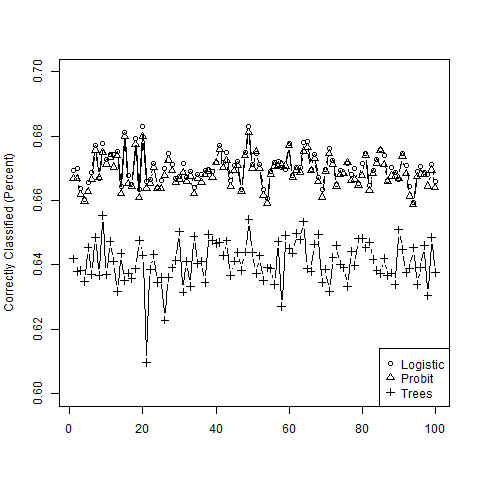
\includegraphics[scale=.7]{this.png}
\end{document}